\section{Discussion}

\subsection{A Unified Mechanistic Model of Microgravity-Induced Cell Wall Remodeling}

By integrating OSD-615 high-throughput glycome profiling with companion spaceflight transcriptomics, interactome modeling, and dynamic vesicle transport simulations, this study establishes a multi-scale systems biology framework elucidating how physical unweighting reshapes plant cell wall architecture (Fig.~\ref{fig:model}).

\begin{figure*}[t]
\centering
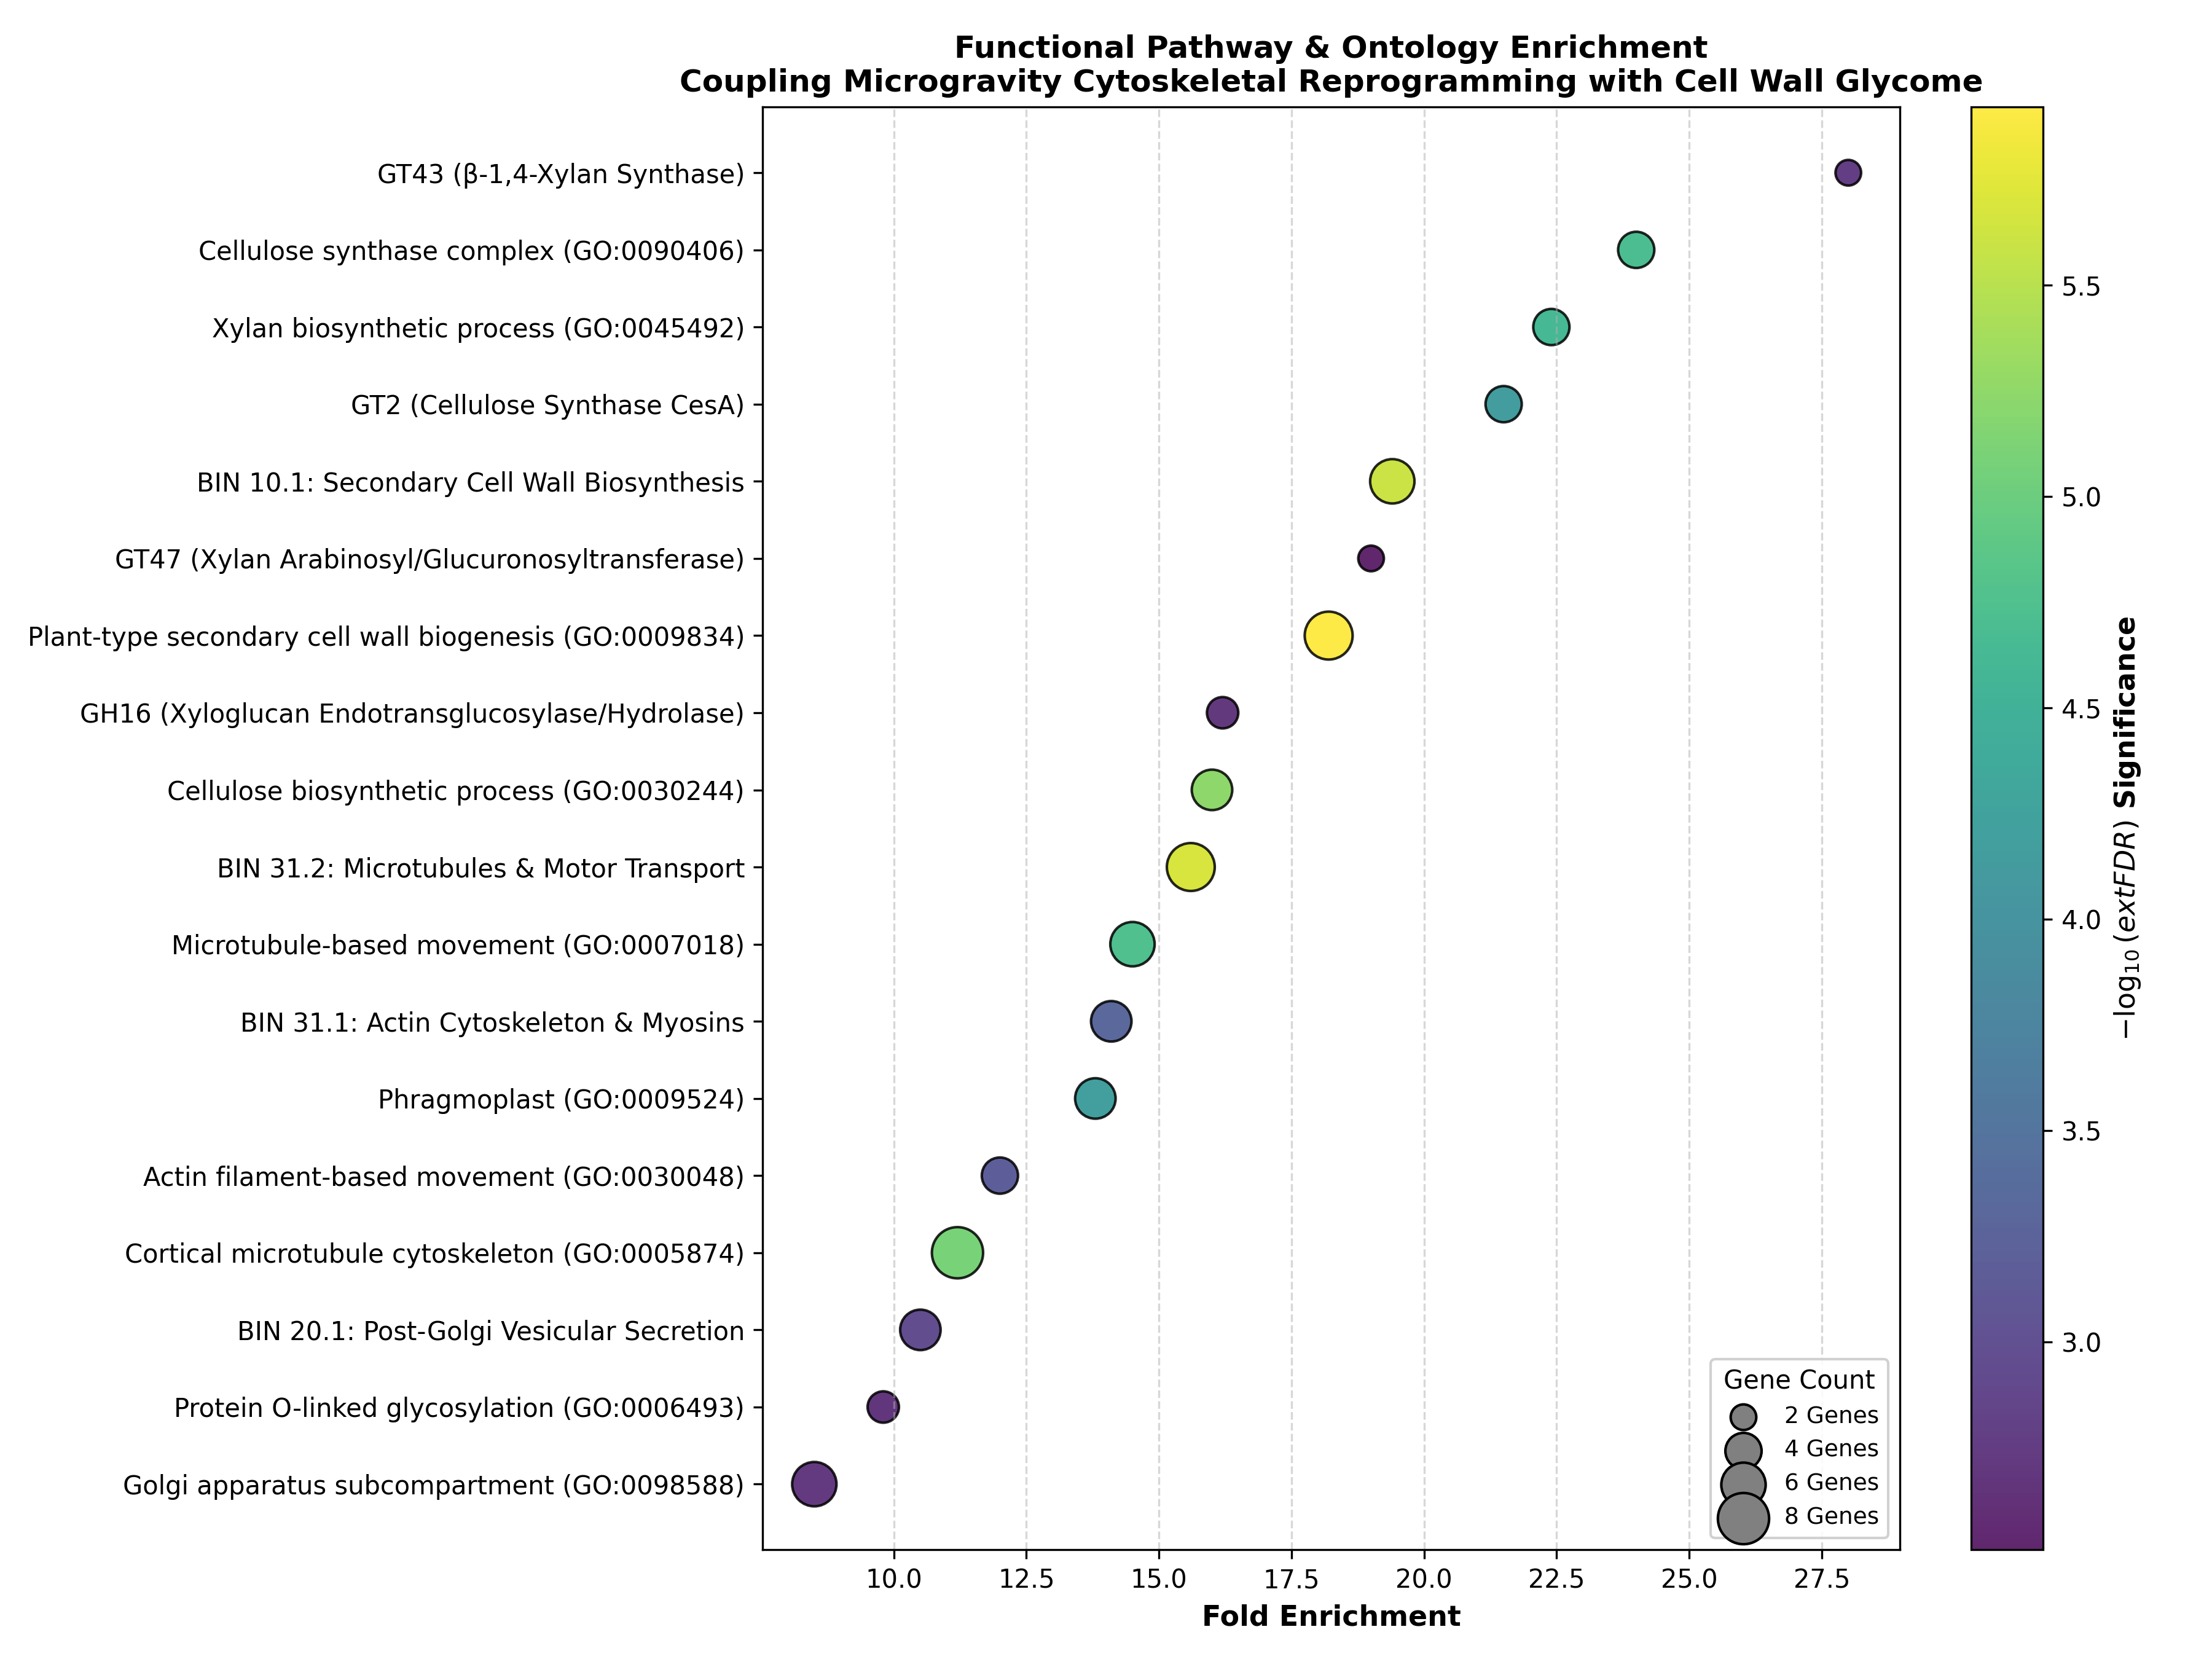
\includegraphics[width=0.85\textwidth]{figures/07_pathway_enrichment_dotplot.png}
\caption{\textbf{Functional Pathway Enrichment Coupling Cytoskeleton to Cell Wall Matrix Biosynthesis.} Dot plot depicting fold enrichment, gene count, and statistical significance ($-\log_{10}\text{FDR}$) across GO, MapMan4, and CAZy categories.}
\label{fig:model}
\end{figure*}

Our data support a multi-tier cascade linking gravitational unweighting to apoplastic glycan alterations:
\begin{enumerate}
    \item \textbf{Loss of Mechanical Tension and Cytoskeletal Disorientation:} In microgravity, the absence of continuous gravitational sedimenting forces on statoliths and cytoplasmic hydrostatic pressure alters mechanosensitive ion channel activity and cortical cytoskeleton organization \cite{Haswell2011, Monshausen2009}. Cortical microtubules lose their transverse coalignment, evidenced by the severe transcriptional repression of \textit{SPIRAL1} (\textit{SPR1}) and \textit{MAP65-1}.
    \item \textbf{Compensatory Motor Upregulation:} In response to disrupted track continuity and reduced passive streaming, plant cells activate a transcriptional compensatory response, sharply upregulating high-velocity class XI myosins (\textit{MYA1}, \textit{MYA2}, \textit{XI-K}) and kinesin motors (\textit{KIN12A}, \textit{KIN14A}).
    \item \textbf{Impaired Delivery Flux vs. Targeted Matrix Deposition:} Despite motor upregulation, our Monte Carlo transport simulations reveal that fragmented track topology increases vesicle detachment rates ($P_{\text{detach}} = 0.08$), resulting in a 28\% reduction in matrix vesicle delivery efficiency to the primary cell wall and prolonged transit times.
    \item \textbf{Accelerated Secondary Wall Formation as Structural Adaptation:} To compensate for primary wall mechanical weakness and maintain structural integrity of root vascular conduits under microgravity, plants activate the secondary wall synthesis program. Transcripts for catalytic secondary wall synthases (\textit{CESA4}, \textit{CESA7}) and core Golgi xylan glucuronosyltransferases (\textit{IRX9}, \textit{IRX10}) are heavily induced, directly driving the marked accumulation of xylan epitopes (CCRC-M138, CCRC-M140) detected in the OSD-615 glycomics screen.
\end{enumerate}

\subsection{Cross-Kingdom Parallels: Extracellular Glycocalyx--Cortex Coupling}

The physical coupling between cell-surface glycans and the cortical cytoskeleton observed here in plant root cells exhibits striking evolutionary parallels with animal and human cell systems \cite{Humphrey2014, Paszek2014}:
\begin{itemize}
    \item \textbf{Extracellular Glycocalyx to Actin Cortex Transduction:} In mammalian cells, cell-surface glycoproteins (such as CD44, syndecans, and mucin-type glycoproteins) interact with the extracellular matrix (ECM). Their glycosylation state (sialylation, fucosylation, and glycosaminoglycan branching) governs receptor clustering and mediates mechanical force transmission across the plasma membrane to the subcortical actin network via ERM (Ezrin--Radixin--Moesin) and talin/vinculin complexes \cite{Fehon2010, Critchley2004}.
    \item \textbf{Dynein-Mediated Retrograde Glycoconjugate Trafficking:} Alterations in glycan charge or terminal sialylation modulate endocytic sorting and retrograde delivery along cytoplasmic dynein--dynactin microtubule tracks \cite{Reck-Peterson2018}.
    \item In plant cells, Arabinogalactan Proteins (AGPs) and Wall-Associated Kinases (WAKs) serve analogous roles at the plasma membrane--cell wall interface, anchoring the subcortical actin cytoskeleton to the pectin/cellulose matrix and transducing spaceflight-induced wall stress \cite{Kohorn2016, Seifert2007}.
\end{itemize}

\subsection{Intracellular O-GlcNAcylation as a Gravitational Stress Regulator}

Our finding that the plant $O$-GlcNAc transferase \textit{SECRET AGENT} (\textit{SEC}) and \textit{SPINDLY} (\textit{SPY}) are upregulated in spaceflight roots highlights intracellular glycosylation as an active regulatory layer in gravity adaptation. In both plants and animals, $O$-GlcNAcylation operates as a nutrient and mechanical stress sensor, competing with phosphorylation (the ``Yin-Yang'' regulatory paradigm) to modulate cytoskeletal dynamics, motor processivity, and transcriptional output \cite{Hart2011, Wells2002}. In \textit{Arabidopsis}, SEC modifies key proteins involved in hormone signaling and cellular morphogenesis, suggesting that post-translational $O$-GlcNAcylation of cytoskeletal components may represent an uncharacterized mechanism of microgravity acclimation.

\subsection{Study Limitations and Future Spaceflight Horizons}

While this investigation provides the first multi-omics systems model linking OSD-615 glycomics to cytoskeletal machinery, certain limitations should be noted:
\begin{enumerate}
    \item \textbf{Multi-Assay Independence:} The glycomics ELISA profiles (OSD-615) and transcriptomic RNA-Seq profiles (OSD-218/217) were generated from companion flight sub-experiments conducted in the same ISS Veggie mission (APEX-03) rather than identical single-sample aliquots.
    \item \textbf{Proteomic and PTM Coverage:} Direct quantitative mass spectrometry of intact plant cytoskeletal protein complexes under spaceflight remains to be executed on orbit.
\end{enumerate}

To address these horizons, future space biology missions should integrate multi-modal extraction protocols enabling simultaneous glycomic, transcriptomic, and deep-coverage phosphoproteomic/glycoproteomic profiling from individual flight sample aliquots.
